\documentclass[12pt,a4paper]{article}
\title{作业114514:逸一时,误一世}
\usepackage{ctex}
\usepackage{amsmath,amscd,amsbsy,amssymb,latexsym,url,bm,amsthm}
\usepackage{epsfig,graphicx,subfigure}
\usepackage{enumitem,balance}
\usepackage{wrapfig}
\usepackage{mathrsfs,euscript}
\usepackage[usenames]{xcolor}
\usepackage{hyperref}
\usepackage[vlined,ruled,commentsnumbered,linesnumbered]{algorithm2e}
\usepackage{float}
\usepackage{geometry}
\geometry{a4paper,scale=0.8}


\title{Lab1 HTML-Parser}
\date{2021.9}
\author{孙济宸\quad 学号:520030910016 \quad 班级:F2003003}
\begin{document}
\maketitle
\section{实验概览}
爬取https://www.baidu.com和https://daily.zhihu.com并且用beautifulsoup库对html文件进行解析,并对其中的各种tag进行查找、筛选并将结果存储在文件中。
\section{实验环境}
\begin{itemize}
	\item Docker
	\item beautifulsoup (bs4)
	\item urllib
	\item re
\end{itemize}
\section{练习题的解决思路}
\subsection{问题1}
问题要求返回网页中所有超链接的URL(不包括图片地址),只要用soup.findAll()方法匹配<a href = “...”>,再用tag.get()方法获取href中内容即可。
\subsection{问题2}
思路同问题一,将匹配的标签变为<img src = "...">,get()获取src中内容即可。
\subsection{问题3}
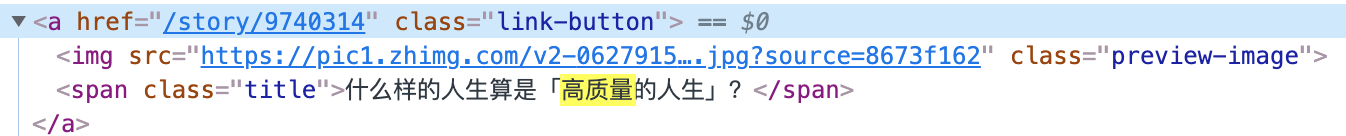
\includegraphics[scale=0.6]{img1.png} \\
通过观察知乎日报的html文件,可以发现日报的每个条目是以<a href = "/story/[日报id]">的格式开始。所以首先用soup.findAll()方法定位所有这个格式的标签;接着对于每个该种标签,
\begin{enumerate}
	\item href中内容即为日报文章url(相对路径)
	\item 子标签0为<img src = "...">,类似问题2获取预览图url
	\item 子标签1为<span class="title">[文章标题]?</span> 通过tag.string方法获取文章标题。
\end{enumerate}
最后将获取到的网页url、图片url及title存进list。
\section{代码运行结果}
\subsection{问题1结果}
完整结果见txt文件
\begin{figure}[H]
	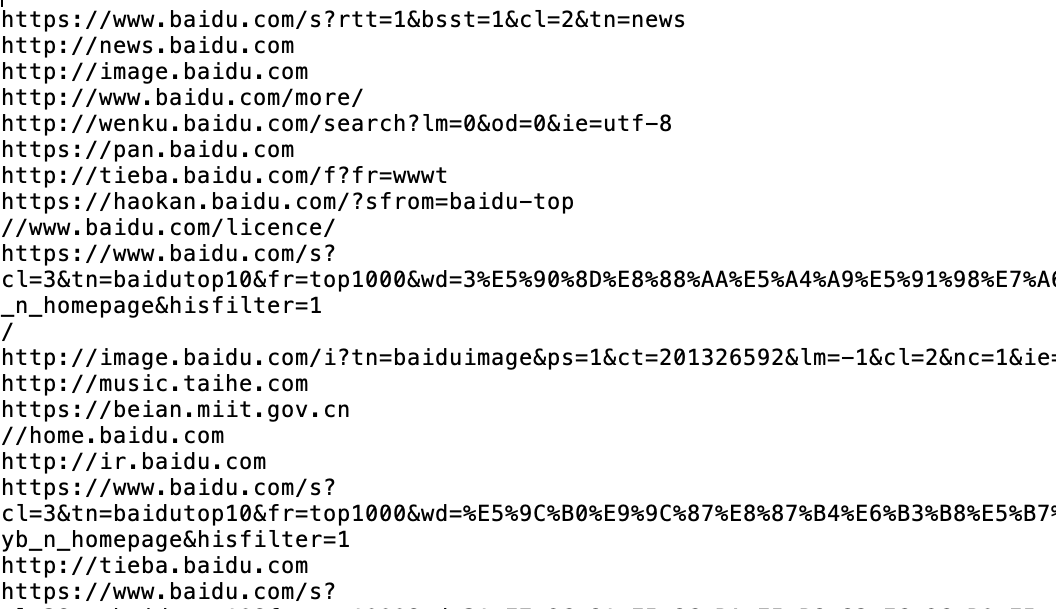
\includegraphics[scale=0.7]{res1.png}
	 \caption{res1.txt}
\end{figure}

\subsection{问题2结果}
\begin{figure}[H]
	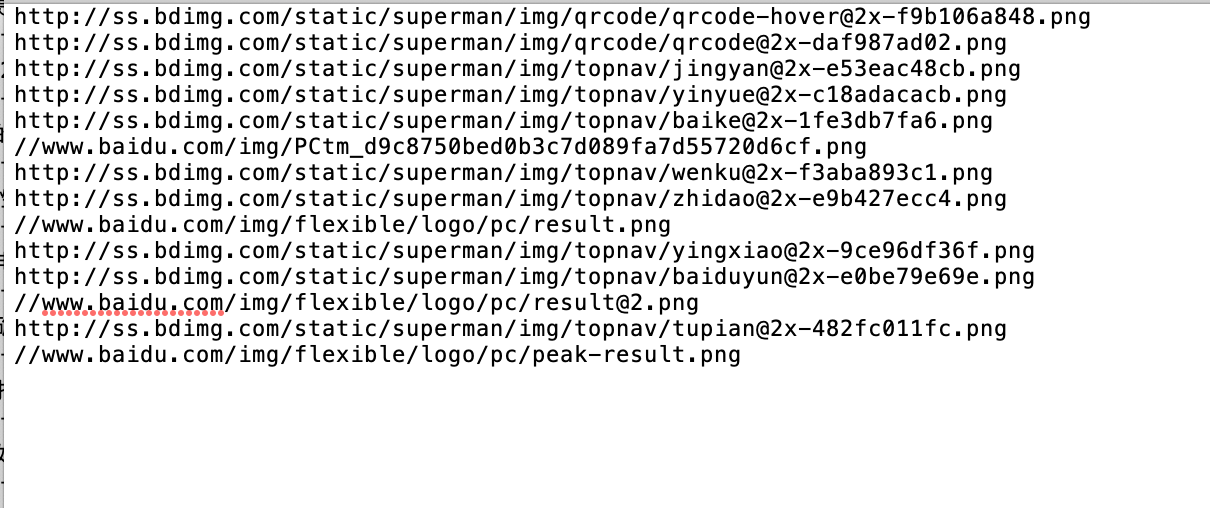
\includegraphics[scale=0.7]{res2.png}
	 \caption{res1.txt}
\end{figure}

\subsection{问题3结果}
\begin{figure}[H]
	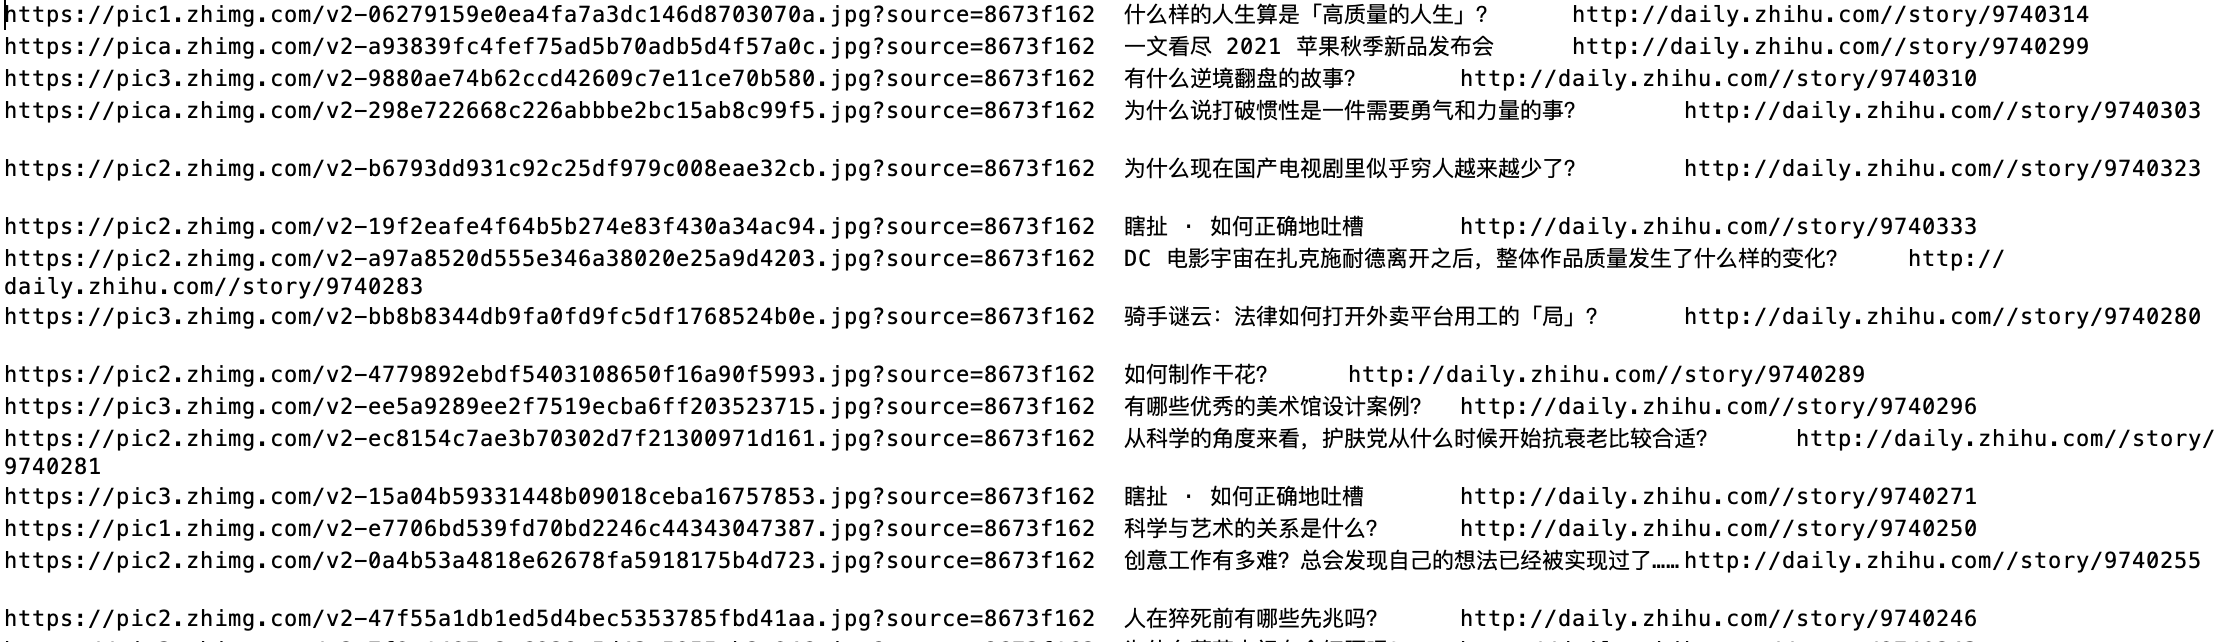
\includegraphics[scale=0.7]{res3.png}
	 \caption{res1.txt}
\end{figure}

\section{分析与思考}
\begin{itemize}
	\item beautifulsoup解析html文件得到的是bs4.BeautifulSoup类型对象; 解析方法如果不指定features = "html.parser",会弹warning。网上资料显示这是默认的解析方法,还可以选择其他的解析方法。
	\item soup.findAll()方法得到一个存有许多标签(tag)的list。这些tag常常是多层嵌套的,可以用parent,contents等多种方法访问。
	\item 问题1中的url有绝对路径、相对路径和javascript等。如果需要进一步处理可能需要分类
	\item tag.find()方法会从这个标签的所有\textbf{子标签}中查找指定内容,并不能查找该标签同层(\textbf{包括自己})的内容!所以问题3中用i.contents[0].find(...)会什么也找不到。这里被坑了好久
	\item 知乎日报文章的标题\textbf{并没有}使用<title>标签,而是用了<span class="title">标签,所以不能直接用tag.title,因此我选择使用tag.string获取标题内容。
\end{itemize}
\end{document}

